\documentclass{llncs}

\usepackage[margin=1in]{geometry}

\usepackage{graphicx,color,comment,url} 

\usepackage{amsmath,amssymb}


\title{[ML20] Assignment 9}
\author{Your Name}
\institute{}

\begin{document}

\maketitle 

\setlength\parindent{0pt} 
\setlength{\parskip}{10pt}

Due: Apr 13 (b 8:45am) 

Let $x \in \mathbb{R}^{p}$ be a random instance 
and $\Sigma_{x} \in \mathbb{R}^{p \times p}$ be 
its covariance matrix. 
Let $w_{1}, w_{2} \in \mathbb{R}^{p}$ be its first 
two optimal PCA projection vectors; we have studied 
how to derive them in the lecture. 

[1] Please derive the third optimal PCA projection 
vector $w_{3}$ by solving (\ref{hw8_eq1}), presuming 
$w_{1}$ and $w_{2}$ are given. Please answer this 
question based on the following three steps. 
\begin{equation}
\label{hw8_eq1}
\max_{w_{3}}\ w_{3}^{T} \Sigma_{x} w_{3} \quad 
s.t.\ ||w_{3}||^{2} = 1,\ cov(w_{3}, w_{1})=0,\ 
cov(w_{3}, w_{2})=0. 
\end{equation}

(i) Show that $cov(w_{3}, w_{1})$=0 is equivalent 
to $w_{3}^{T} w_{1}$=0, and $cov(w_{3}, w_{2})$=0 
is equivalent to $w_{3}^{T} w_{2}$=0. 

(ii) In order to apply Lagrange Multiplier to 
solve (\ref{hw8_eq1}), we need to first construct 
the Lagrange function
\begin{equation}
\label{hw8_eq2}
J = w_{3}^{T} \Sigma_{x} w_{3} 
+ \lambda_{1} (w_{3}^{T} w_{3} - 1)
+ \lambda_{2} (w_{3}^{T} w_{1}) 
+ \lambda_{3} (w_{3}^{T} w_{2}). 
\end{equation}
Show that $\lambda_{2} = 0$ and $\lambda_{3} = 0$. 

(iii) Optimize $J$ over $w_{3}$ and show the 
optimal $w_{3}$ is an eigenvector of $\Sigma_{x}$. 
(Need to show derivatives.) 
 
\newpage 

Implement PCA and apply it to learn 
$p$ projection vectors $w_{1}, w_{2}, \ldots, w_{p-1}, w_{p}$ from a set 
of instances $x_{1}, x_{2}, \ldots, x_{n} 
\in \mathbb{R}^{p}$. Assume these
projection vectors are sorted as follows: 
$w_{1}$ is associated with the largest eigenvalue, $w_{2}$ with the second 
largest, ..., and $w_{p}$ with the 
smallest eigenvalue. 

[2] Plot the distribution of these 
instances in a 2D feature space in 
two figures. 
In Fig \ref{hw9_fig1}, the two latent 
features are generated through $w_{1}$ 
and $w_{2}$. In Fig 2, the two are
generated through $w_{p-1}$ and $w_{p}$. 

\begin{figure}[h!] 
\centering 
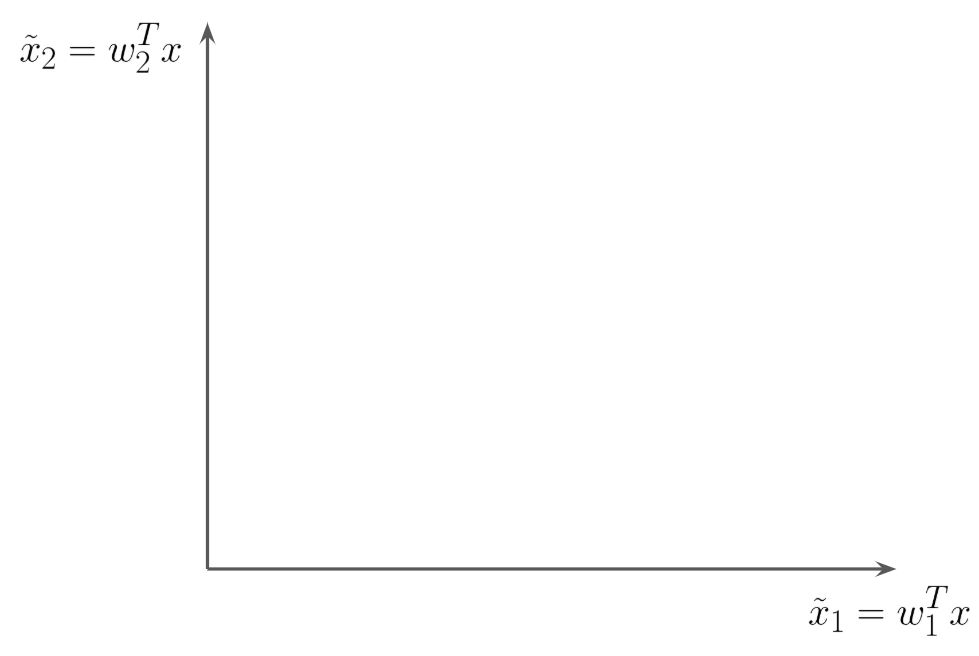
\includegraphics[width=.6\textwidth]{assignment/hw9_fig1.jpg} 
\caption{Data Distribution based 
on $w_{1}$ and $w_{2}$.} 
\label{hw9_fig1}
\end{figure}

\begin{figure}[h!] 
\centering 
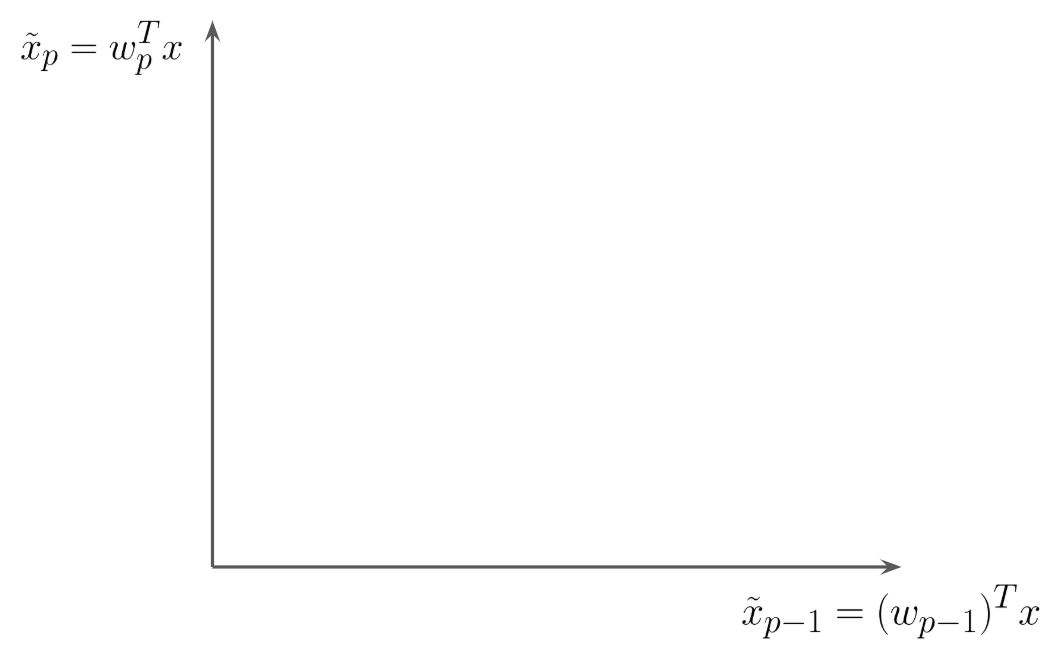
\includegraphics[width=.6\textwidth]{assignment/hw9_fig2.jpg} 
\caption{Data Distribution based 
on $w_{p-1}$ and $w_{p}$.} 
\label{hw9_fig2}
\end{figure}

\newpage 

Continue [2]. 
Let us train a prediction model 
in the PCA projected space and evaluate 
its performance. Draw your results as a curve in Fig \ref{hw9_fig3}, where 
x-axis is $k$ and y-axis is testing mse.

For the prediction task, let $x_{1},
\ldots, x_{n}$ be a set of training instances, and $t_{1}, \ldots, t_{m}$ 
be a set of testing instances -- 
keep in mind they are all 
$p$-dimensional feature vectors, 
and their labels are assumed given. 
Let $\tilde{x} \in \mathbb{R}^{k}$ 
be the latent feature vector
of an arbitrary instance $x$ 
(training or testing) generated trough 
\begin{equation}
\label{hw9_eq3}
\tilde{x} = 
\begin{bmatrix}
w_{1}^{T} x\\
w_{2}^{T} x\\
\vdots\\ 
w_{k}^{T} x 
\end{bmatrix} \in \mathbb{R}^{k}. 
\end{equation}

For each choice of $k$, we can 
follow the following steps to 
get the testing mse. 

(i) Train a set of optimal  
PCA projection vectors $w_{1}, 
w_{2}, \ldots, w_{k}$ from the 
\textit{training set}. (Done 
in [2].)

(ii) Obtain a set of projected 
training instances 
$\tilde{x}_{1}, \tilde{x}_{2}, \ldots, 
\tilde{x}_{n} \in \mathbb{R}^{k}$, 
where $\tilde{x}_{i}$ is the latent 
feature vector of $x_{i}$ obtained 
through (\ref{hw9_eq3}). 

(iii) Train a linear regression $f$
model on $\tilde{x}_{1}, \tilde{x}_{2}, \ldots, \tilde{x}_{n}$ and their labels. 
(Note that labels are untouched.)  

(iv) Obtain a set of projected 
testing instances 
$\tilde{t}_{1}, \tilde{t}_{2}, \ldots, 
\tilde{t}_{n} \in \mathbb{R}^{k}$, 
where $\tilde{t}_{i}$ is the latent 
feature vector of $t_{i}$ obtained 
through (\ref{hw9_eq3}). 

(v) Apply $f$ on $\tilde{t}_{1}, \tilde{t}_{2}, \ldots, \tilde{t}_{n}$ 
to predict their labels and estimate 
testing mse. (Question: 
why on the projected testing instances? 
Can we directly evaluate $f$ on the
original testing instances?) 

Note: choose 5 values of $k$ yourself 
and try to make the curve as convergent 
as possible. (Think about how mse may 
behave when $k$ is extremely small or 
extremely large.) 


\begin{figure}[h!] 
\centering 
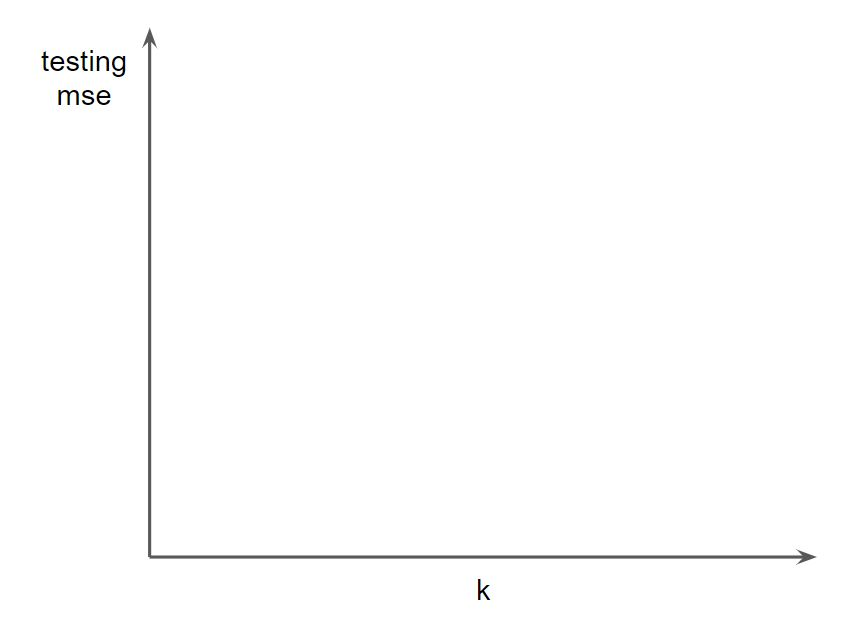
\includegraphics[width=.6\textwidth]{assignment/hw9_fig3.jpg} 
\caption{Data Distribution based 
on $w_{p-1}$ and $w_{p}$.} 
\label{hw9_fig3}
\end{figure}

\newpage 

[4] (Bonus) 
Kernel PCA is a nonlinear dimensionality reduction technique, which first maps 
data into a higher dimensional space, 
and then finds an optimal PCA projection
vector in that space. However, since 
the mapping is implicit, kernel PCA needs
to apply the Representer theorem and kernel
trick to derive an analytic solution 
for the optimal projection vector. 

Let's verify the Representer theorem. 
Let $x_{1}, \ldots, x_{n}$ be a set 
of instances and $\Sigma_{x}$ be their 
covariance matrix. Let $w$ be the optimal 
PCA projection vector learned from 
this set. Please show that $w$ can 
be written as 
\begin{equation}
w = \sum_{i = 1}^{n} \alpha_{i} 
\bar{x}_{i}, 
\end{equation}
where $\alpha_{i}$'s are unknown
coefficients and $\bar{x}_{i}$ 
is a `centered' instance of $x_{i}$ 
defined as 
\begin{equation}
\bar{x}_{i} = x_{i} -
\frac{1}{n}\sum_{j=1}^{n} x_{j}. 
\end{equation}
Tip: recall the optimal PCA project 
vector satisfies 
$\Sigma_{x} w = \lambda w$.

\newpage 

[5] (Bonus) Let us try to mathematically 
develop a variant of CCA. For a pair of 
variables $x$ and $z$, suppose we want 
to find a pair of projection vectors 
$w$ and $v$ such that the covariance 
(not correlation) between these variables
in the projected space  is maximized. 
In addition, you are NOT allowed to use 
the constraints that 
$var(w^{T}x) = c_{1}$ and 
$var(v^{T}z) = c_{2}$ (or their 
square-roots), where $c_{1}$ and $c_{2}$ 
are constants. 

Please derive the optimal $w$ and 
$v$. If necessary, design 
your own constraints that do not 
violate the above requirements. 
Eventually, you may just show $w$ 
and $v$ are generalized eigenvectors 
of some problem. 

\end{document}

